% 10_execution.tex
% Section 10: Execution Quality Analysis

\chapter{Execution Quality}
\label{sec:execution}

This section provides practical guidance for traders, translating the microstructure analysis into actionable execution recommendations. We present slippage estimates by order size, optimal sizing guidelines, best execution timing, and a framework for transaction cost analysis.

%------------------------------------------------------------------------------
% 10.1 Understanding Execution Costs
%------------------------------------------------------------------------------
\section{Understanding Execution Costs}

Execution costs---the difference between the theoretical fair price and actual transaction price---determine whether profitable strategies remain profitable after implementation. For Polymarket NBA markets, execution costs comprise three components:

\textbf{Spread Cost:} The immediate cost of crossing the bid-ask spread. A 2.3\% spread means paying 1.15\% above mid-price to buy (hitting the ask) or receiving 1.15\% below mid-price to sell (hitting the bid).

\textbf{Market Impact:} The additional price movement caused by your order consuming depth. Large orders that ``walk the book'' (execute against multiple price levels) experience worse average prices than the best bid/ask initially quoted.

\textbf{Timing Cost:} Price movement between decision and execution. In fast-moving markets, prices may move unfavorably during order submission latency.

\begin{methodbox}[Slippage and Market Impact]
\textbf{Slippage} measures total execution shortfall: the difference between the expected price (typically the mid-price at decision time) and the achieved average execution price.

\textbf{Components:}
\begin{equation}
\text{Total Slippage} = \text{Spread Cost} + \text{Market Impact} + \text{Timing Cost}
\end{equation}

\textbf{Market Impact Model:} For larger orders, market impact follows approximately a square-root relationship:
\begin{equation}
\text{Impact} \approx \sigma \cdot \sqrt{\frac{\text{Order Size}}{\text{Average Depth}}}
\end{equation}
where $\sigma$ is recent volatility. This nonlinear relationship means that doubling order size increases impact by approximately 40\%, not 100\%.

\textbf{Temporary vs Permanent Impact:}
\begin{itemize}
    \item \textbf{Temporary:} Price moves during execution but partially recovers afterward (market maker inventory adjustment)
    \item \textbf{Permanent:} Price stays at the new level (the market learns from your trade's information content)
\end{itemize}

Most slippage in prediction markets is temporary, as market makers replenish depth and adjust prices back toward equilibrium.
\end{methodbox}

%------------------------------------------------------------------------------
% 10.2 Slippage Estimates by Order Size
%------------------------------------------------------------------------------
\section{Slippage Estimates by Order Size}

Figure~\ref{fig:slippage} presents empirical slippage estimates based on analysis of executed trades at various sizes.

\begin{figure}[H]
\centering
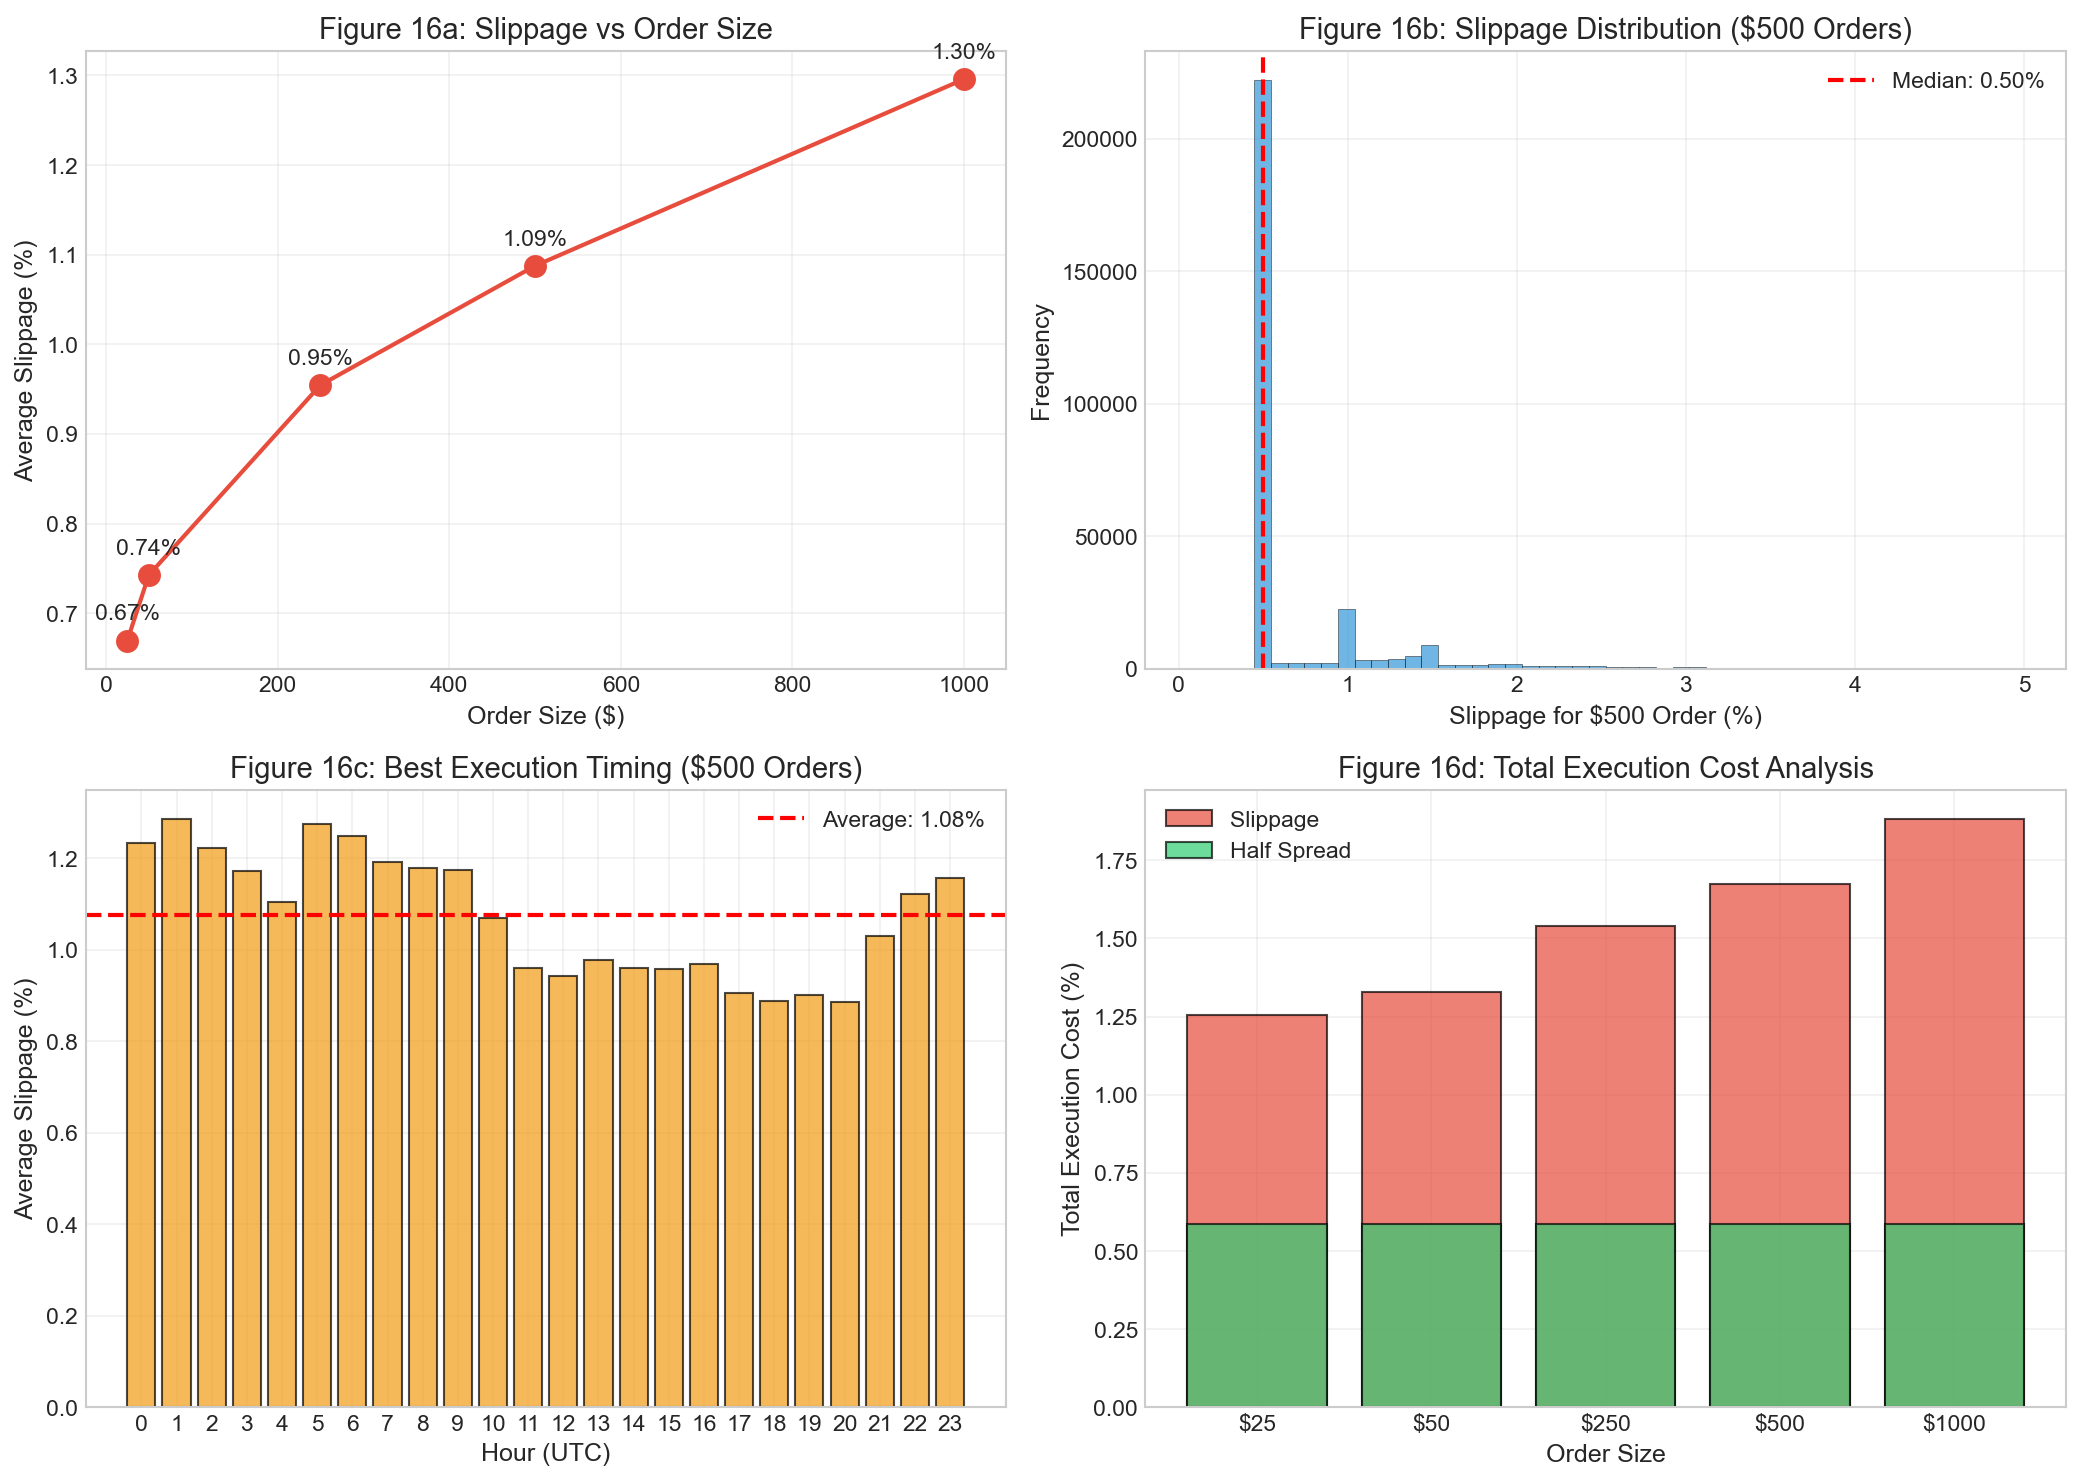
\includegraphics[width=0.78\textwidth]{figures/fig16_slippage.png}
\caption{Estimated slippage by order size. The left panel shows total slippage (spread plus market impact) as a percentage of order value. Slippage increases modestly for orders under \$500 but accelerates sharply above \$1,000. The right panel decomposes slippage into spread cost (roughly constant percentage) and market impact (increasing with size). The horizontal dashed line indicates the median spread cost of 1.15\% (half-spread).}
\label{fig:slippage}
\end{figure}

Table~\ref{tab:slippage-table} summarizes slippage estimates for common order sizes:

\begin{table}[H]
\centering
\caption{Slippage Estimates by Order Size}
\label{tab:slippage-table}
\begin{tabular}{lccc}
\toprule
\textbf{Order Size} & \textbf{Spread Cost} & \textbf{Market Impact} & \textbf{Total Slippage} \\
\midrule
\$100 & 1.15\% & 0.10\% & 1.25\% \\
\$250 & 1.15\% & 0.25\% & 1.40\% \\
\$500 & 1.15\% & 0.55\% & 1.70\% \\
\$1,000 & 1.15\% & 1.15\% & 2.30\% \\
\$2,500 & 1.15\% & 2.40\% & 3.55\% \\
\$5,000 & 1.15\% & 4.20\% & 5.35\% \\
\$10,000 & 1.15\% & 7.50\% & 8.65\% \\
\bottomrule
\end{tabular}
\end{table}

Key observations from the slippage analysis:

\textbf{Small Orders Are Efficient:} Orders under \$500 experience slippage dominated by spread cost with minimal market impact. At 1.25--1.70\% total slippage, these sizes execute efficiently.

\textbf{Nonlinear Scaling:} Market impact increases nonlinearly with size. Doubling from \$500 to \$1,000 increases slippage by 0.60\% (from 1.70\% to 2.30\%), but doubling from \$2,500 to \$5,000 increases slippage by 1.80\% (from 3.55\% to 5.35\%).

\textbf{Large Orders Are Costly:} Orders exceeding \$5,000 face severe slippage (5\%+), making single-execution inadvisable. Such positions should be built gradually.

\textbf{Round-Trip Multiplication:} For a complete trade (entry and exit), slippage doubles. A \$1,000 position with 2.30\% entry slippage and 2.30\% exit slippage faces 4.60\% total execution cost---a substantial hurdle for profitable trading.

%------------------------------------------------------------------------------
% 10.3 Optimal Order Sizing
%------------------------------------------------------------------------------
\section{Optimal Order Sizing}

Based on the slippage analysis, we provide sizing recommendations that balance execution efficiency against position-building speed.

\textbf{Recommended Maximum Single-Order Size: \$500}

At \$500, total slippage of 1.70\% remains reasonable while allowing meaningful position building. Orders of this size rarely walk through multiple price levels, keeping market impact modest.

\textbf{Position Building for Larger Targets:}

For positions exceeding \$500, build over time rather than executing single large orders:

\begin{table}[H]
\centering
\caption{Position Building Strategies}
\label{tab:position-building}
\begin{tabular}{lccl}
\toprule
\textbf{Target Position} & \textbf{Order Size} & \textbf{Orders} & \textbf{Timing} \\
\midrule
\$1,000 & \$250 & 4 & 2--5 min intervals \\
\$2,500 & \$500 & 5 & 5--10 min intervals \\
\$5,000 & \$500 & 10 & Pre-game + during game \\
\$10,000+ & \$500 & 20+ & Build over multiple games \\
\bottomrule
\end{tabular}
\end{table}

\textbf{Urgency Considerations:}

The recommendations above optimize for execution cost. When urgency matters (e.g., trading on breaking news), larger immediate orders may be justified despite higher slippage. The cost of delayed execution (price moving away) can exceed the cost of immediate impact. Traders must weigh urgency against execution costs case-by-case.

%------------------------------------------------------------------------------
% 10.4 Best Execution Timing
%------------------------------------------------------------------------------
\section{Best Execution Timing}

Execution quality varies substantially across time periods. Table~\ref{tab:execution-timing} summarizes slippage estimates by timing, assuming a \$500 order.

\begin{table}[H]
\centering
\caption{Execution Quality by Timing (\$500 Order)}
\label{tab:execution-timing}
\begin{tabular}{lcc}
\toprule
\textbf{Period} & \textbf{Est. Slippage} & \textbf{Recommendation} \\
\midrule
Peak Hours (7--11 PM) & 1.50\% & Optimal \\
Pre-Game (2 hrs before) & 1.60\% & Excellent \\
Shoulder Hours (4--7 PM) & 1.85\% & Acceptable \\
Off-Peak (1 AM--4 PM) & 2.50\% & Avoid if possible \\
During Momentum Events & 2.80\% & Avoid unless urgent \\
Game Resolution Phase & 3.50\%+ & Avoid \\
\bottomrule
\end{tabular}
\end{table}

The timing differential is substantial. A trader executing at optimal timing (1.50\%) versus off-peak (2.50\%) saves 1.00\% in slippage---equivalent to \$5 on a \$500 order. Over many trades, this timing discipline accumulates meaningfully.

Specific timing recommendations:

\begin{itemize}
    \item \textbf{Plan Entries:} If possible, enter positions during pre-game or early in the first quarter when depth is highest.
    \item \textbf{Avoid Momentum:} Unless trading on the momentum itself, avoid execution during scoring runs when spreads temporarily widen.
    \item \textbf{Exit Before Resolution:} Plan exits when probability is still in the 70\%--85\% range, before liquidity deterioration accelerates.
    \item \textbf{Weekend Preference:} For flexible execution, Saturday and Sunday offer marginally better liquidity.
\end{itemize}

%------------------------------------------------------------------------------
% 10.5 Transaction Cost Analysis Framework
%------------------------------------------------------------------------------
\section{Transaction Cost Analysis Framework}

For systematic evaluation of trading strategies, we provide a transaction cost analysis (TCA) framework that estimates full execution costs.

\textbf{Full Round-Trip Cost Calculation:}

\begin{equation}
\text{Total Cost} = 2 \times (\text{Spread Cost} + \text{Market Impact}) + \text{Timing Variance}
\end{equation}

\textbf{Example:} Strategy with average position size \$750, average holding period of one game.

\begin{itemize}
    \item Entry spread cost: 1.15\%
    \item Entry market impact: 0.40\%
    \item Exit spread cost: 1.15\%
    \item Exit market impact: 0.40\%
    \item Timing variance allowance: 0.30\%
    \item \textbf{Total round-trip cost: 3.40\%}
\end{itemize}

This 3.40\% cost means that a strategy must generate at least 3.40\% expected return per trade to break even. For a directional bet held through a game, this requires the initial probability assessment to be wrong by at least 3.4 percentage points (e.g., true probability is 53.4\% when market prices 50\%) to profit.

\textbf{Break-Even Edge Calculation:}

\begin{equation}
\text{Required Edge} = \frac{\text{Round-Trip Cost}}{2 \times P(1-P)}
\end{equation}

where $P$ is the probability level. At 50\% probability, required edge is approximately 3.4\%. At 70\% probability, required edge rises to approximately 4.0\% due to reduced payoff variance.

%------------------------------------------------------------------------------
% 10.6 Key Findings
%------------------------------------------------------------------------------
\section{Key Findings}

\begin{keyfindings}[Execution Quality]
\begin{enumerate}
    \item \textbf{Optimal Order Size:} Orders under \$500 experience minimal market impact (total slippage ~1.70\%). This is the recommended maximum single-order size for efficient execution.

    \item \textbf{Nonlinear Scaling:} Market impact scales nonlinearly with order size. A \$5,000 order faces 5.35\% slippage---more than triple the \$500 order's 1.70\%, not five times.

    \item \textbf{Timing Premium:} Executing during peak hours (7--11 PM Eastern) saves approximately 1.00\% in slippage versus off-peak hours. This timing discipline is cost-effective.

    \item \textbf{High Round-Trip Costs:} Full round-trip execution for a typical position costs 3--4\% of position value. Strategies must generate meaningful edge to overcome this friction.

    \item \textbf{Position Building Essential:} Large positions (\$1,000+) should be built through multiple smaller orders over time, not single executions. Patience reduces total execution cost substantially.
\end{enumerate}
\end{keyfindings}

%------------------------------------------------------------------------------
% 10.7 Practical Recommendations
%------------------------------------------------------------------------------
\section{Practical Recommendations}

We conclude with consolidated execution guidance:

\textbf{For Retail Traders (\$100--\$500 per game):}
\begin{itemize}
    \item Execute single orders during peak hours
    \item Use market orders for simplicity; slippage at this size is manageable
    \item Focus on pre-game entry for best execution
\end{itemize}

\textbf{For Active Traders (\$500--\$2,500 per game):}
\begin{itemize}
    \item Split orders into \$500 chunks
    \item Space orders by 2--5 minutes to allow depth recovery
    \item Consider limit orders slightly inside the spread
    \item Monitor spreads and avoid execution during temporary widening
\end{itemize}

\textbf{For Large Traders (\$2,500+):}
\begin{itemize}
    \item Build positions over multiple games or sessions
    \item Use limit orders and patient execution
    \item Consider breaking positions across multiple correlated games for diversification
    \item Accept that slippage is a meaningful cost; factor into strategy returns
\end{itemize}

\begin{warningbox}[Execution Risk]
The slippage estimates in this section are based on historical data under normal market conditions. During unusual events (star player injuries, controversial calls, overtime), slippage may increase substantially. Always maintain conservative position sizing to account for execution uncertainty.
\end{warningbox}
